%%%%%%%%%%%%%%%%%%%%%%%%%%%%%%%%%%%%%%%%%%%%%%%%%%%%%%%%%%%%%%%%%%%%
% Poster template for Master Projects
% Creation: September 17, 2008
% Modified: October 10, 2008
% Authors: Erik Steur and Rob Mestrom (WH -1.144)
%%%%%%%%%%%%%%%%%%%%%%%%%%%%%%%%%%%%%%%%%%%%%%%%%%%%%%%%%%%%%%%%%%%%

\documentclass[12pt,a4paper]{article}
\usepackage[a4,wtbuk,themedarkblue]{tuepdfscreen2008}
\usepackage[english]{babel}
\usepackage{amsmath,amssymb}
%\usepackage{mathtime}     % This package is not required, it loads Mathtime fonts for mathematical formulas which I prefer.
%\usepackage{framed}         % Used for textboxes
%\usepackage{wrapfig}        % Used to wrap figures
\usepackage{graphicx}
\usepackage{enumitem}
\usepackage[font=footnotesize,labelfont=bf]{caption}
\usepackage{lipsum}

%% For posterboxes?
%\usepackage[orientation=portrait,size=a4,scale=1.0]{beamerposter}

\usepackage[tikz]{bclogo}
\renewcommand \logowidth{0pt}
\newcommand{\emptylogo}{
\includegraphics[width=0pt]{Figures/Empty}}

%% To turn Figure into Fig.
%\renewcommand{\figurename}{Fig.}
%\addto\captionsenglish{\renewcommand{\figurename}{Fig.}}

%\usepackage[framemethod=tikz]{mdframed}
%\usepackage[style=1]{mdframed}
%\newcommand\Loadedframemethod{TikZ}
%\usepackage[framemethod=\Loadedframemethod]{mdframed}
%\newmdtheoremenv [
%    outerlinewidth = 2 ,
%    leftmargin = 40 ,
%    rightmargin = 40 ,
%    backgroundcolor = yellow ,
%    outerlinecolor = blue ,
%    innertopmargin = \topskip ,
%    splittopskip = \topskip ,
%    ntheorem = true ,
%    skipabove = \baselineskip ,
%    skipbelow = \baselineskip ]
%    {theorem}{Theorem}[section]

%% Tikz
%\usepackage{tikz}
%\usetikzlibrary{backgrounds}


%%%%%%%%%%%%%%%%%%%%%%%%%%%%%%%%%%%%%%%%%%%%%%%%%%%%%%%%%%%%%%%%%%%%
% Correct hyphenation
%%%%%%%%%%%%%%%%%%%%%%%%%%%%%%%%%%%%%%%%%%%%%%%%%%%%%%%%%%%%%%%%%%%%
\hyphenation{off-line}

%%%%%%%%%%%%%%%%%%%%%%%%%%%%%%%%%%%%%%%%%%%%%%%%%%%%%%%%%%%%%%%%%%%%
% Modify itemize
%%%%%%%%%%%%%%%%%%%%%%%%%%%%%%%%%%%%%%%%%%%%%%%%%%%%%%%%%%%%%%%%%%%%
%[itemsep = 0pt, parsep = 0pt]
%\newenvironment{my_itemize}{
%\begin{itemize}
%  \setlength{\topsep}{0pt}
%  \setlength{\leftmargin}{-0.5cm}%{0pt}
%  \setlength{\itemindent}{0pt}%{-0.5cm}%{0pt}
%  \setlength{\parindent}{-0.5cm}%{0pt}
%  \setlength{\itemsep}{0pt}
%  \setlength{\parskip}{0pt}
%  \setlength{\parsep}{0pt}}
%{\end{itemize}
%}
%\setlist[itemize]{noitemsep, topsep=0pt, leftmargin=-0.5cm, itemindent=-0.5cm, parindent=-0.5cm, itemsep=0pt, parskip=0pt, parsep=0pt}

%%%%%%%%%%%%%%%%%%%%%%%%%%%%%%%%%%%%%%%%%%%%%%%%%%%%%%%%%%%%%%%%%%%%
% Logos and title layout
%%%%%%%%%%%%%%%%%%%%%%%%%%%%%%%%%%%%%%%%%%%%%%%%%%%%%%%%%%%%%%%%%%%%

% Insert company logo (max height approximately 14 mm)
%% PDF
\setstatustext{
\includegraphics[height=14mm]{Figures/logoAtHome.pdf}\hspace{1.5cm}
\includegraphics[height=14mm]{Figures/GO_2017}}

%% DVI
%\setstatustext{
\includegraphics[height=14mm, bb = 0 0 458 266]{Figures/logoAtHome.png}\hspace{3.0cm}\includegraphics[height=14mm,bb = 0 0 670 175]{Figures/RoboCup2013logo.png}}
% If no company logo is needed, uncomment the following line
%\setstatustext{}

%\Committee{
\includegraphics[height=35mm]{Figures/techunitedlogo} }
\Committee{
    
\includegraphics[height=44mm]{Figures/techunitedlogo}
}
\Sponsors{
    
\includegraphics[width=50mm]{Figures/Vanderlande_logo}
\\
\\
    
\includegraphics[width=50mm]{Figures/SKM_logo}
}

\begin{document}
\begin{slidetop}

%%%%%%%%%%%%%%%%%%%%%%%%%%%%%%%%%%%%%%%%%%%%%%%%%%%%%%%%%%%%%%%%%%%%
% [Author] and {Title} of the poster
%%%%%%%%%%%%%%%%%%%%%%%%%%%%%%%%%%%%%%%%%%%%%%%%%%%%%%%%%%%%%%%%%%%%
\slidetitle[RoboCup~German~Open~2017]{\vspace{10mm} Tech United Eindhoven}

\begin{multicols}{2}

\begin{bclogo}[couleur = white, arrondi = 0.25, couleurBord = tuedarkblue , barre = none, logo=\emptylogo]{\textcolor{tuedarkblue}{AMIGO \& SERGIO}}
\medskip %\bigskip
\begin{minipage}[T]{0.48\linewidth}
	\begin{center}
		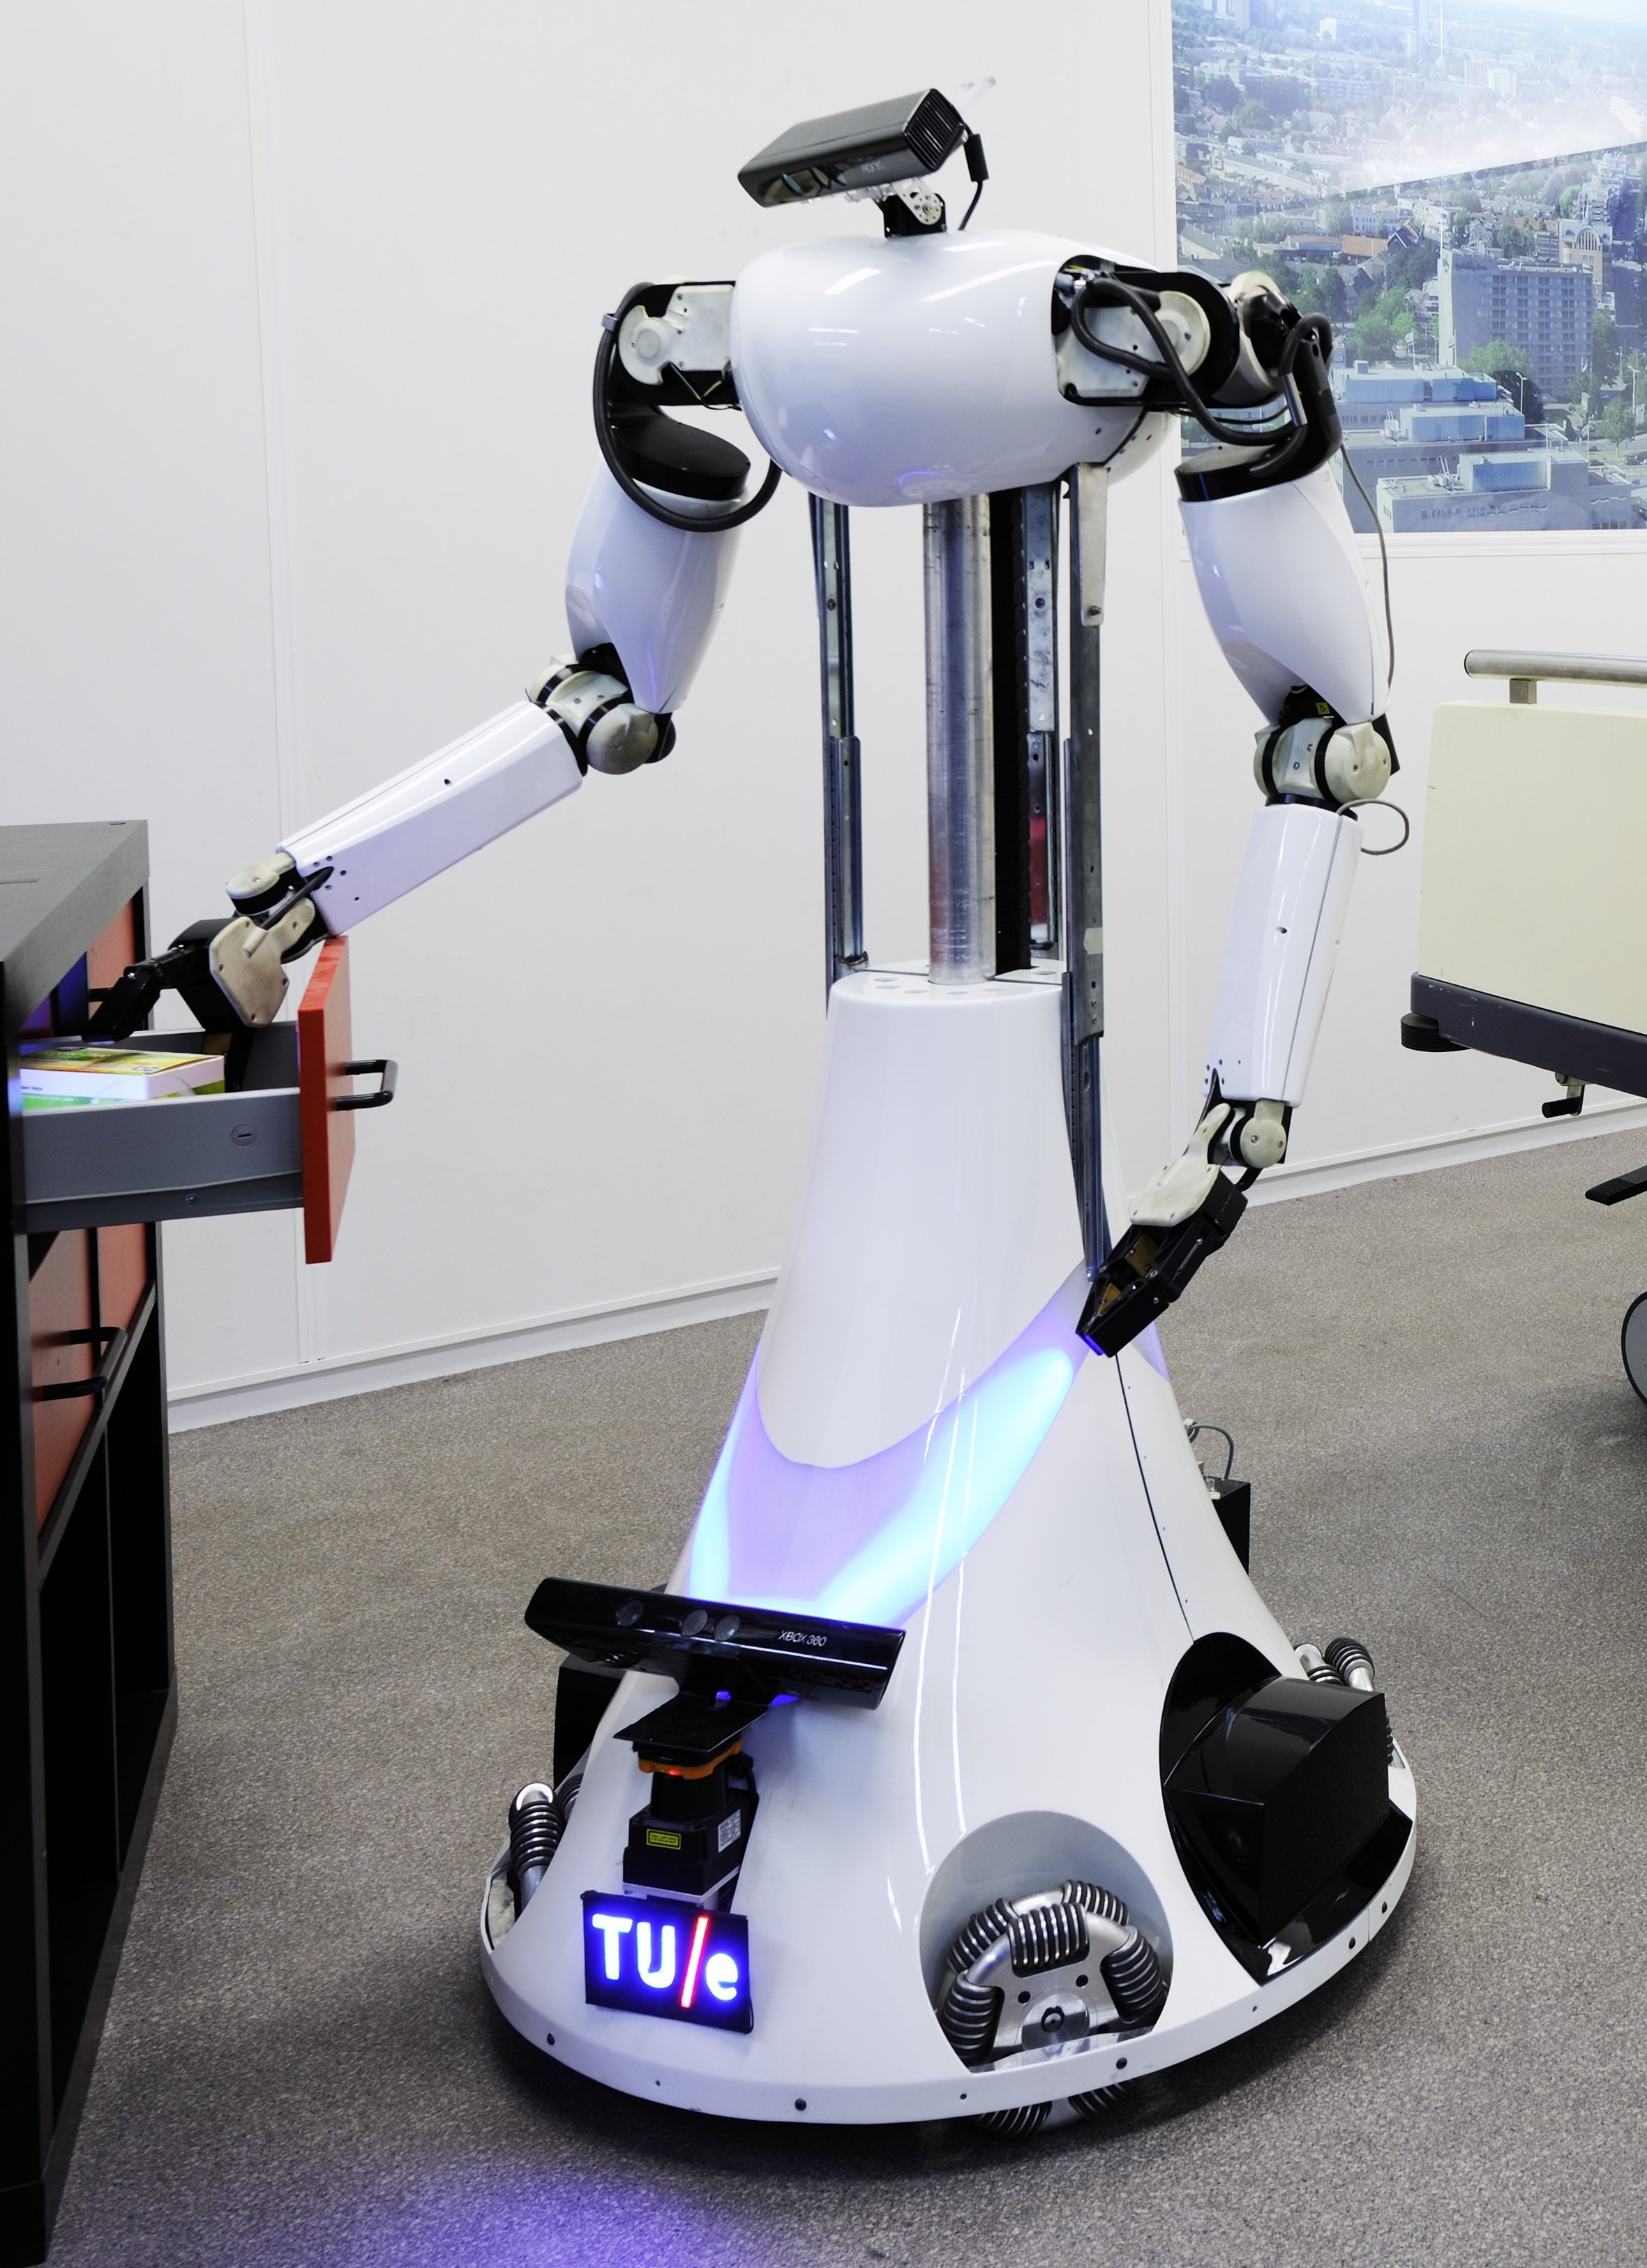
\includegraphics[height=4cm]{Figures/amigo_hospital72}
		\figcaption{AMIGO\the\premulticols}
	\end{center}
\end{minipage}
\hfill
\begin{minipage}[T]{0.48\linewidth}
    \begin{center}
    	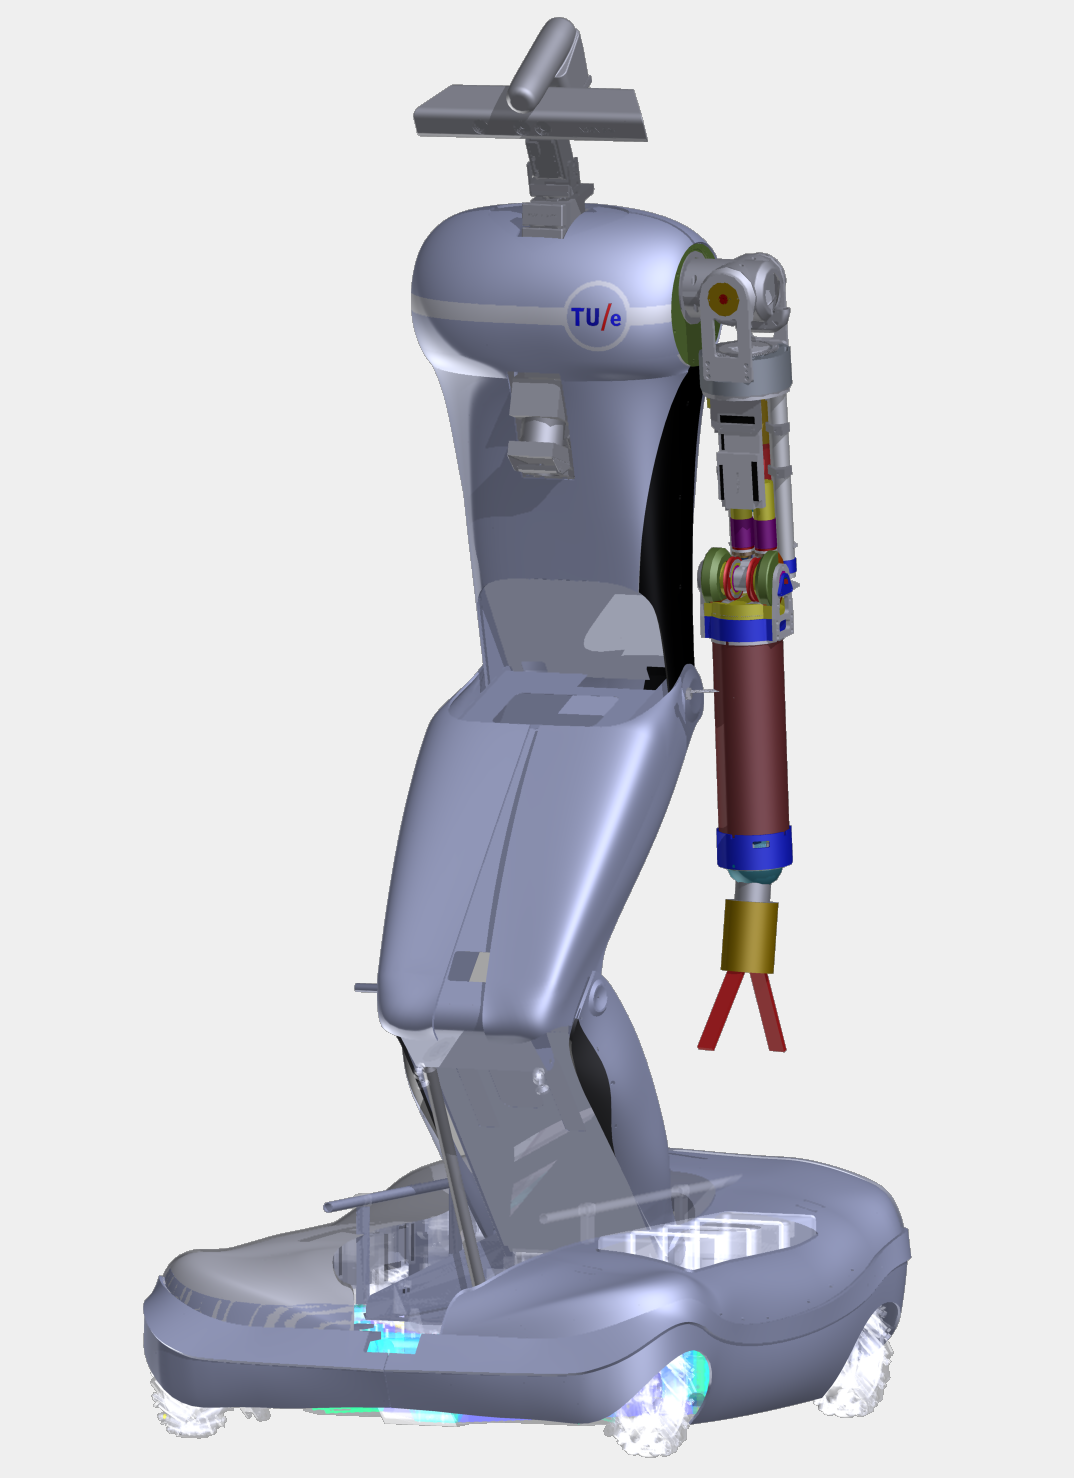
\includegraphics[height=4cm]{Figures/SERGIO}
        \figcaption{SERGIO}
    \end{center}
\end{minipage}
    \begin{itemize}[itemsep = 0pt, parsep = 0pt, leftmargin=15pt]
    	\item AMIGO
    	\begin{itemize}[itemsep = 0pt, parsep = 0pt, leftmargin=15pt]
    		\item Omni-wheels, 1 DoF torso
    	\end{itemize}
    	\item SERGIO
    	\begin{itemize}[itemsep = 0pt, parsep = 0pt, leftmargin=15pt]
    		\item Suspended mecanum wheels, 2 DoF torso
    	\end{itemize}
        \item 7-DoF manipulators
        \item Designs available at Robotic Open Platform
    \end{itemize}
\end{bclogo}

%\vspace{0.2cm}
\vspace{-0.8cm} % remove when compiling on linux

\begin{bclogo}[couleur = white, arrondi = 0.25, couleurBord = tuedarkblue , barre = none, logo=\emptylogo]{\textcolor{tuedarkblue}{Improved manipulation}}
\medskip %\bigskip
\begin{minipage}[T]{0.48\textwidth}
    \begin{center}
        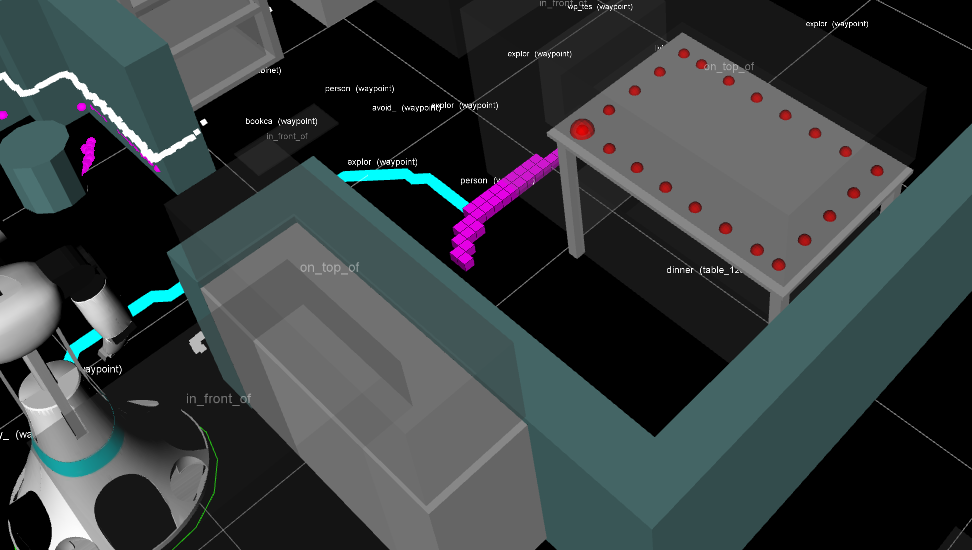
\includegraphics[width=\linewidth]{Figures/manipulation_emtpy_spot}
    \end{center}
\end{minipage}
\hfill
\begin{minipage}[T]{0.48\textwidth}
    \begin{center}
        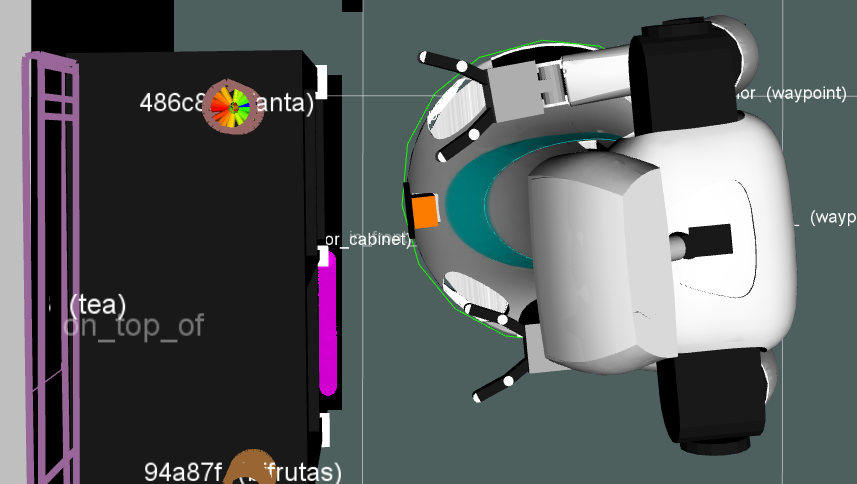
\includegraphics[width=1\linewidth]{Figures/manipulation_grasp_point}
    \end{center}
\end{minipage}
\begin{itemize}[itemsep = 0pt, parsep = 0pt, leftmargin=15pt]
	\item Empty spot designator
    \begin{itemize}[itemsep = 0pt, parsep = 0pt, leftmargin=15pt]
		\item Incorporating current position
	\end{itemize}
	\item Grasping point determination
\end{itemize}
\end{bclogo}

%\vspace{0.2cm}
\vspace{-0.8cm} % remove when compiling on linux

\begin{bclogo}[couleur = white, arrondi = 0.25, couleurBord = tuedarkblue , barre = none, logo=\emptylogo]{\textcolor{tuedarkblue}{Image recognition}}
\medskip %\bigskip
\begin{minipage}[T]{\textwidth}
    \begin{center}
        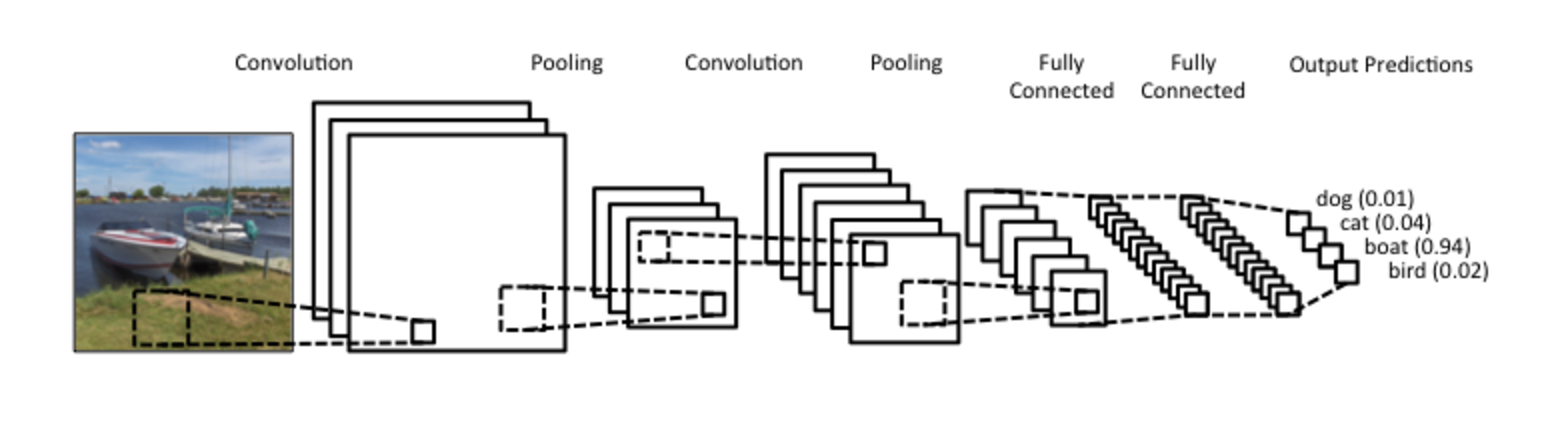
\includegraphics[width=0.9\linewidth]{Figures/cnn}
    \end{center}
\end{minipage}
\begin{itemize}[itemsep = 0pt, parsep = 0pt, leftmargin=15pt]
	\item Object recognition using Deep Learning
	\item Face recognition: Openface based on Torch
    \item ROS-packages: ros-kinetic-image-recognition
    \begin{itemize}[itemsep = 0pt, parsep = 0pt, leftmargin=15pt]
		\item Including training and test GUIs
	\end{itemize}
\end{itemize}
\end{bclogo}

%\vspace{-0.4cm}
\vfill
\columnbreak
% end of left column

\begin{bclogo}[couleur = white, arrondi = 0.25, couleurBord = tuedarkblue , barre = none, logo=\emptylogo]{\textcolor{tuedarkblue}{World modeling}}
\medskip %\bigskip
\begin{minipage}[T]{\textwidth}
    \begin{center}
        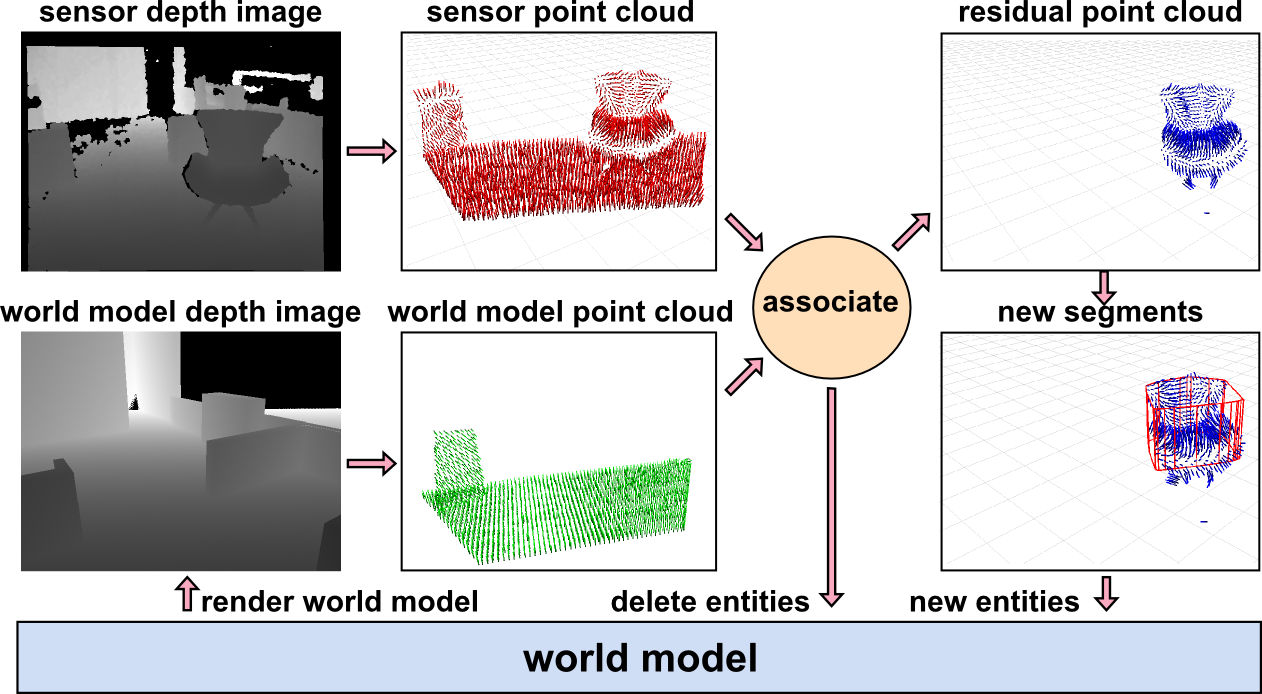
\includegraphics[width=0.9\linewidth]{Figures/ed_pipeline}
	\figcaption{Overview of ED: Environment Descriptor}
    \end{center}
\end{minipage}
\begin{itemize}[itemsep = 0pt, parsep = 0pt, leftmargin=15pt]
	\item A central object-oriented, volumetric world model, used for:	
	\begin{itemize}[itemsep = 0pt, parsep = 0pt, leftmargin=15pt]
		\item Navigation, localization
		\item Object tracking
	\end{itemize}
	\item Objects have 3D shape, pose, type
	\item Updating by comparing rendered world model with depth image
    \item Furniture fitting
    \begin{itemize}[itemsep = 0pt, parsep = 0pt, leftmargin=15pt]
		\item Increases performance of navigation, localisation and object segmentation
	\end{itemize}


\end{itemize}
\end{bclogo}

%\vspace{0.2cm}
\vspace{-0.83cm} % remove when compiling on linux

\begin{bclogo}[couleur = white, arrondi = 0.25, couleurBord = tuedarkblue , barre = none, logo=\emptylogo]{\textcolor{tuedarkblue}{WebGUI}}
\medskip %\bigskip
\begin{minipage}[T]{\textwidth}
    \begin{center}
        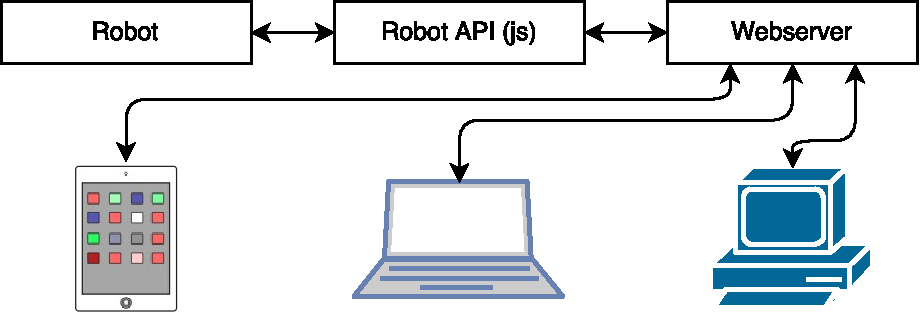
\includegraphics[width=0.9\linewidth]{Figures/webgui_architecture}
%        \figcaption{
%		 Overview of the WebGUI architecture.
%		 The robot's functionalities are exposed with the Robot API that is implemented in JavaScript.
%		 The webserver that is hosting the GUI connects this Robot API to a graphical user interface that is offered to multiple clients on different platforms.}
%	      \label{fig:webgui_architecture}
    \end{center}
\end{minipage}
\begin{itemize}[itemsep = 0pt, parsep = 0pt, leftmargin=15pt]
	\item Web-based Graphical User Interface
	\item Cross-platform
	\item Action server schedules the robot's tasks based on user input
\end{itemize}
\end{bclogo}

%\vspace{0.2cm}
\vspace{-0.83cm} % remove when compiling on linux

\begin{bclogo}[couleur = white, arrondi = 0.25, couleurBord = tuedarkblue, barre = none, logo=\emptylogo]{\textcolor{tuedarkblue}{Natural language interpretation}}
\medskip %\bigskip
\begin{itemize}[itemsep = 0pt, parsep = 0pt, leftmargin=15pt]
	\item Natural Language Interpretation using Feature Context Free Grammar
	\item Speech recognition grammars are deduced from the NLI grammars
\end{itemize}
\end{bclogo}


\includegraphics[width=0pt]{Figures/Empty}
\end{multicols}
\end{slidetop}

\end{document}

